\documentclass[11pt,a4paper]{article}

\usepackage[T1]{fontenc}
\usepackage{helvet}
\renewcommand{\familydefault}{\sfdefault}
\renewcommand{\ttdefault}{\sfdefault}
\usepackage[top=2cm, bottom=2cm, left=2cm, right=2cm]{geometry}
\usepackage{amsmath}
\usepackage{amssymb}
\usepackage{graphicx}
\usepackage{booktabs}
\usepackage{hyperref}
\usepackage{cite}
\usepackage{float}
\usepackage{parskip}

\hypersetup{colorlinks=true,linkcolor=blue,citecolor=blue,urlcolor=blue}

\title{\textbf{COMP0240 Challenge CW1: Structural Inspection Path Planning}\\
\large Autonomous Systems and Robotics}
\author{Ali Shihab \\ \texttt{ali.shihab.25@ucl.ac.uk}}
\date{April 2026}

\begin{document}
\maketitle

% ─────────────────────────────────────────────────────────────────────────────
\section{Problem Statement and Objectives}
% ─────────────────────────────────────────────────────────────────────────────

Autonomous structural inspection requires a UAV to visit a set of predefined viewpoints, each tagged with an ArUco fiducial marker that confirms visual coverage, while avoiding cuboid obstacles~\cite{bircher2015structural}. Given a scenario file specifying obstacle geometry and viewpoint poses $(x, y, z, \text{yaw})$, the system must compute a collision-free flight plan and prove completion by photographing every marker.

It splits into two coupled sub-problems: a \emph{tour ordering} problem, a variant of the Travelling Salesman Problem~\cite{lawler1985travelling}, fixing the sequence of viewpoints; and a \emph{local motion planning} problem computing safe trajectories between them. Four scenarios vary viewpoint count (5--20) and obstacle count (1--10). My objectives were to (i) reach every viewpoint and confirm its marker, (ii) keep clear of obstacles, (iii) minimise tour time and path distance, (iv) log enough evidence to audit completion, and (v) attribute any improvement to a specific component rather than to the system as a whole.

% ─────────────────────────────────────────────────────────────────────────────
\section{Methodology}
% ─────────────────────────────────────────────────────────────────────────────

\subsection{Algorithm Selection}

\textbf{Tour ordering.} File order produces tours that cross themselves repeatedly (Figure~\ref{fig:paths}, left panel). Nearest-neighbour construction~\cite{lawler1985travelling} with 2-opt refinement~\cite{croes1958method} runs offline before any flight command. Edge weights are straight-line Euclidean distance rather than true obstacle-aware path length: computing the latter needs $O(n^2)$ planner invocations to build the cost matrix (190 for 20 viewpoints) before the drone leaves the ground. Euclidean weights underestimate edges passing through obstacles, so ordering is slightly optimistic in cluttered scenes, but the approximation is cheap and the resulting tours proved good enough that the error never dominated.

\textbf{A\textsuperscript{*} local planning.} Straight-line execution flies the drone into obstacles when a viewpoint sits behind one. A 3D A\textsuperscript{*} planner~\cite{hart1968formal} over a voxel grid with obstacle inflation replaces this. A\textsuperscript{*} was preferred to Dijkstra~\cite{dijkstra1959note} because the Euclidean heuristic expands far fewer nodes in these mostly-open scenarios at no cost to optimality. A greedy line-of-sight pass~\cite{daniel2010theta} then drops intermediate grid waypoints wherever a direct free segment exists. I dropped Dubins paths~\cite{dubins1957curves} on kinematic grounds: a multirotor has no minimum turning radius and can yaw on the spot, so a Dubins model imposes a constraint the vehicle does not have.

\textbf{RRT\textsuperscript{*} local planning.} RRT\textsuperscript{*} samples directly in continuous $\mathbb{R}^3$~\cite{karaman2011sampling,lavalle1998rapidly} and converges asymptotically on the optimal path, which should give shorter, less angular routes than a grid can express.

\subsection{Experimental Design}

My first evaluation compared three configurations: straight-line with file ordering, A\textsuperscript{*} with NN+2-opt, and RRT\textsuperscript{*} with NN+2-opt. Only after collecting it did I notice the design is confounded. Ordering and local planner change together, so no difference can be attributed to either, and since reordering shortens a tour while obstacle detours lengthen it, the two effects partly cancel.

I rebuilt it as a \textbf{full $2\times3$ factorial}: ordering $\in$ \{file order, NN+2-opt\} $\times$ planner $\in$ \{straight, A\textsuperscript{*}, RRT\textsuperscript{*}\}, on all four scenarios, three repeats, giving 24 cells and 72 runs. Holding one factor constant isolates the other, and the repeats give a variance estimate, without which a few seconds cannot be told from noise.

\subsection{System Architecture and Parameters}

The same scenario YAML drives both simulator and planner. A generator expands it into a Gazebo world, emitting one SDF box per obstacle and an ArUco marker 1\,m in front of each viewpoint along its yaw axis, so planner geometry and flown geometry cannot diverge. Aerostack2 (AS2)~\cite{fernandez2023aerostack2} spawns the quadrotor and exposes the behaviour interface.

The planner parses the same YAML, builds the occupancy grid, and computes the tour and all local paths \emph{offline} before streaming waypoints to the AS2 \texttt{GoTo} action server. No planning occurs in flight, so planning cost never appears in any timing metric. Obstacle avoidance is consequently a design-time property: obstacles are inflated by 0.4\,m when the grid is built and every waypoint issued is already known to be clear. There is no reactive avoidance, which is acceptable for a static, fully-mapped environment but would not be for an unmapped structure.

A verification thread polls TF at 10\,Hz and marks a viewpoint reached once the tolerances in Table~\ref{tab:params} are met. Marker detection runs OpenCV \texttt{aruco}~\cite{garrido2014automatic} on the onboard camera stream. Watchdogs bound every blocking action: a leg is abandoned after 20\,s without positional progress, and the arm, offboard and takeoff calls each carry an explicit timeout. Each run writes a timestamped directory containing the pose trajectory sampled at a pinned 50\,Hz, a JSONL event log recording every arrival, tolerance check and marker detection with timestamps, and a metrics summary. Every figure in this report traces back to those logs.

\begin{table}[H]
\centering\small
\caption{Parameters, identical across all 72 runs.}
\label{tab:params}
\begin{tabular}{llll}
\toprule
\textbf{Parameter} & \textbf{Value} & \textbf{Parameter} & \textbf{Value} \\
\midrule
Commanded speed    & 3.0\,m/s   & RRT\textsuperscript{*} rewire radius & 2.0\,m \\
Voxel resolution   & 0.5\,m     & RRT\textsuperscript{*} goal bias     & 15\,\% \\
Obstacle inflation & 0.4\,m     & RRT\textsuperscript{*} iterations    & 3000 / segment \\
Position tolerance & 0.75\,m    & Watchdog stall timeout               & 20\,s \\
Yaw tolerance      & 30$^\circ$ & Trajectory sampling                  & 50\,Hz \\
Dwell at viewpoint & 0.2\,s     & ArUco inspection window              & 5\,s \\
\bottomrule
\end{tabular}
\end{table}

% ─────────────────────────────────────────────────────────────────────────────
\section{Results and Discussion}
% ─────────────────────────────────────────────────────────────────────────────

Table~\ref{tab:results} reports all 24 cells as mean $\pm$ s.d.\ over three runs. \emph{Success} is the fraction of runs reaching every viewpoint; \emph{ArUco} is the fraction of viewpoints whose marker was positively identified. Six further runs failed in the harness (a wedged simulator startup) and were retried rather than recorded, since such a failure reflects the test rig, not the planner.

\begin{table}[H]
\centering\footnotesize
\caption{Factorial results, $n=3$. \emph{Tour}: takeoff to final viewpoint. \emph{Total}: takeoff to touchdown. Bold = best tour time per scenario. $^\dagger$Not comparable: an incomplete run flies less because it does less.}
\label{tab:results}
\begin{tabular}{llrrrrrr}
\toprule
\textbf{Sc} & \textbf{Ordering / Planner} & \textbf{Tour (s)} & \textbf{Total (s)} & \textbf{Path (m)} & \textbf{Cover} & \textbf{ArUco} & \textbf{Success} \\
\midrule
1 & File order / Straight & 107.3\,$\pm$\,2.9 & 129.8 & 153.9\,$\pm$\,0.5 & 100\% & 97\% & 100\% \\
  & File order / A*       & 129.9\,$\pm$\,2.6 & 153.0 & 158.8\,$\pm$\,0.2 & 100\% & 100\% & 100\% \\
  & File order / RRT*     & 116.2\,$\pm$\,6.3 & 139.0 & 156.8\,$\pm$\,0.6 & 100\% & 97\% & 100\% \\
  & NN+2-opt / Straight   & \textbf{93.5}\,$\pm$\,17.5 & 119.5 & 91.1\,$\pm$\,0.8 & 100\% & 93\% & 100\% \\
  & NN+2-opt / A*         & 98.7\,$\pm$\,7.3 & 121.6 & 95.8\,$\pm$\,0.2 & 100\% & 100\% & 100\% \\
  & NN+2-opt / RRT*       & 95.1\,$\pm$\,8.3 & 120.5 & 93.4\,$\pm$\,1.0 & 100\% & 90\% & 100\% \\
\midrule
2 & File order / Straight$^\dagger$ & 170.3 & 206.5 & 105.4 & 53\% & 50\% & \textbf{0\%} \\
  & File order / A*       & 136.2\,$\pm$\,1.3 & 159.2 & 156.0\,$\pm$\,0.2 & 100\% & 100\% & 100\% \\
  & File order / RRT*     & 164.7\,$\pm$\,14.1 & 188.4 & 154.9\,$\pm$\,0.1 & 100\% & 93\% & 100\% \\
  & NN+2-opt / Straight   & \textbf{88.9}\,$\pm$\,7.8 & 115.2 & 91.3\,$\pm$\,1.5 & 100\% & 100\% & 100\% \\
  & NN+2-opt / A*         & 111.1\,$\pm$\,3.7 & 137.3 & 95.7\,$\pm$\,0.7 & 100\% & 97\% & 100\% \\
  & NN+2-opt / RRT*       & 107.0\,$\pm$\,4.7 & 133.1 & 95.2\,$\pm$\,1.7 & 100\% & 87\% & 100\% \\
\midrule
3 & File order / Straight & 201.1\,$\pm$\,9.8 & 227.2 & 217.6\,$\pm$\,0.4 & 100\% & 93\% & 100\% \\
  & File order / A*       & 241.5\,$\pm$\,10.5 & 266.5 & 226.2\,$\pm$\,1.8 & 100\% & 93\% & 100\% \\
  & File order / RRT*     & 243.1\,$\pm$\,25.2 & 267.6 & 226.7\,$\pm$\,2.7 & 100\% & 93\% & 100\% \\
  & NN+2-opt / Straight   & \textbf{136.6}\,$\pm$\,21.8 & 162.1 & 110.0\,$\pm$\,1.2 & 100\% & 97\% & 100\% \\
  & NN+2-opt / A*         & 162.7\,$\pm$\,8.6 & 188.5 & 118.8\,$\pm$\,0.8 & 100\% & 100\% & 100\% \\
  & NN+2-opt / RRT*       & 154.9\,$\pm$\,5.8 & 180.7 & 118.5\,$\pm$\,0.6 & 100\% & 98\% & 100\% \\
\midrule
4 & File order / Straight$^\dagger$ & 90.6 & 115.0 & 64.6 & 60\% & 53\% & 33\% \\
  & File order / A*       & \textbf{77.3}\,$\pm$\,1.3 & 100.9 & 73.7\,$\pm$\,0.8 & 100\% & 100\% & 100\% \\
  & File order / RRT*$^\dagger$ & 103.7 & 129.0 & 71.6 & 87\% & 87\% & 67\% \\
  & NN+2-opt / Straight$^\dagger$ & 77.3 & 100.0 & 64.8 & 67\% & 67\% & \textbf{0\%} \\
  & NN+2-opt / A*         & \textbf{73.4}\,$\pm$\,7.1 & 96.0 & 70.7\,$\pm$\,0.7 & 100\% & 93\% & 100\% \\
  & NN+2-opt / RRT*       & 74.7\,$\pm$\,3.0 & 97.6 & 70.0\,$\pm$\,1.2 & 100\% & 100\% & 100\% \\
\bottomrule
\end{tabular}
\end{table}

\begin{figure}[H]
  \centering
  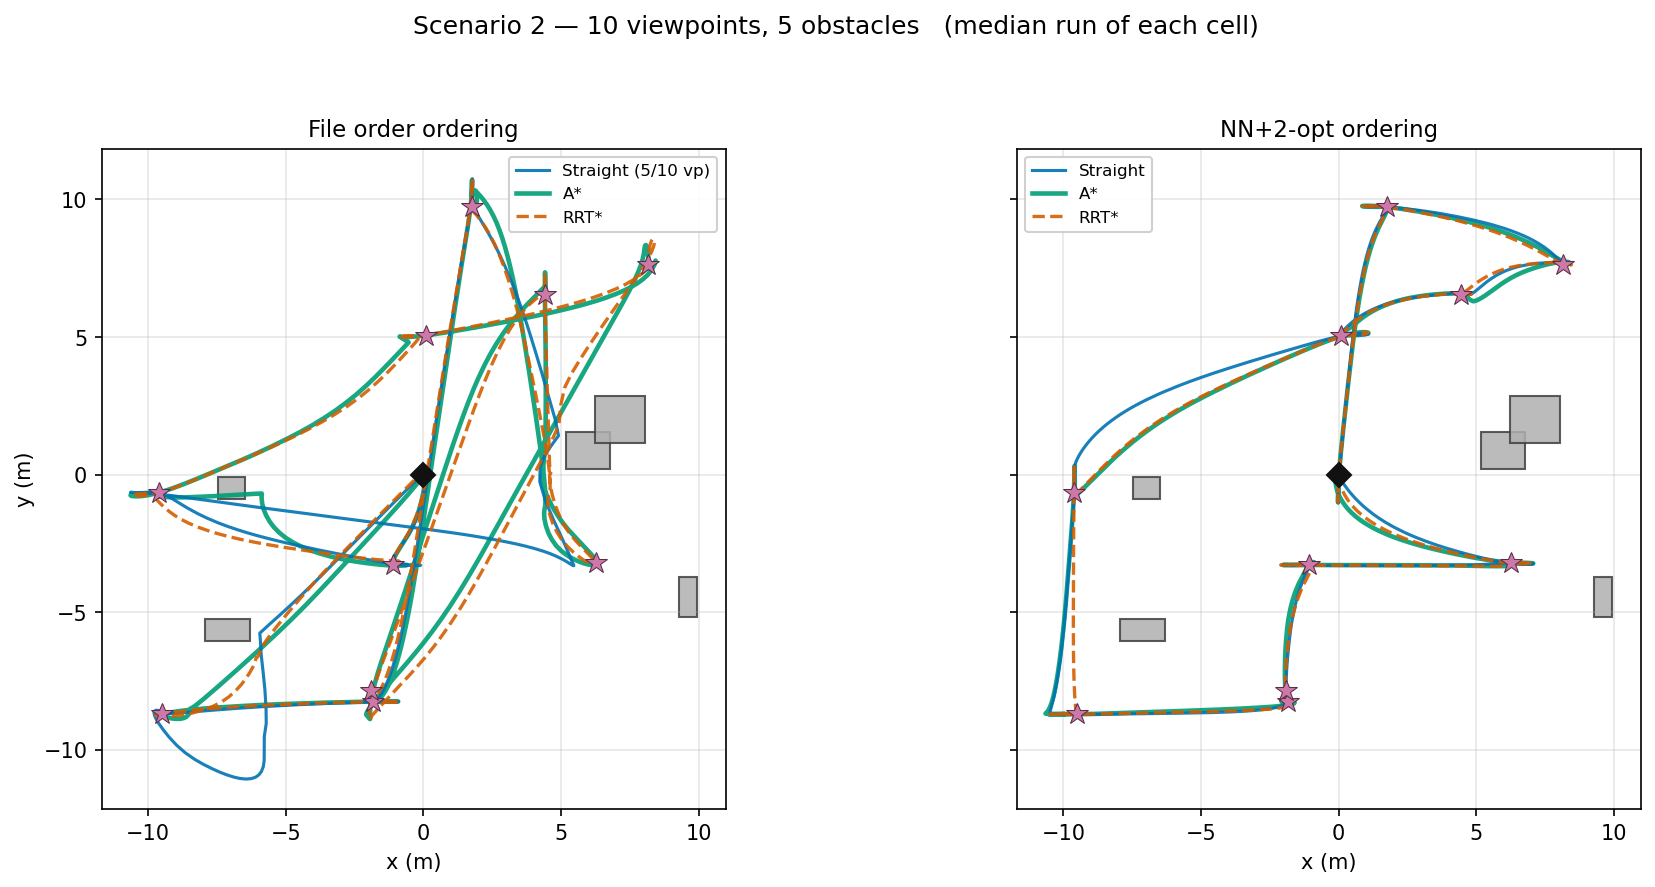
\includegraphics[width=0.49\textwidth]{report_figs/fig_paths_scenario2.png}
  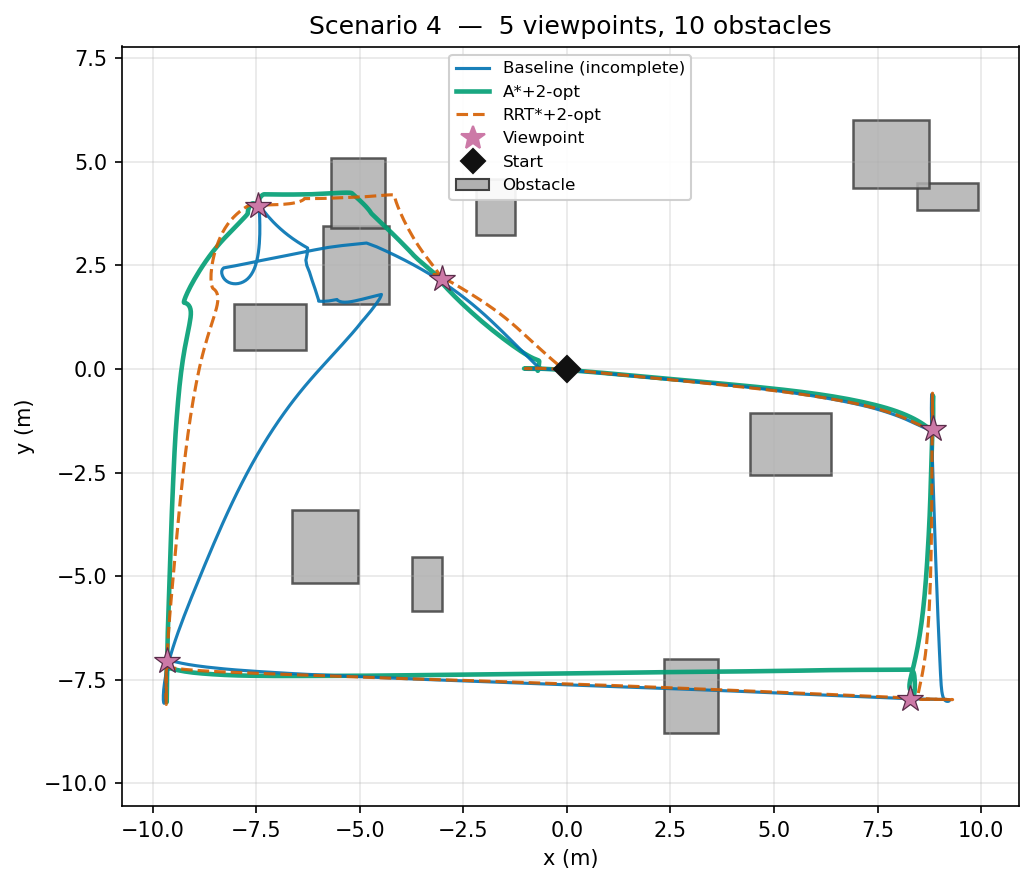
\includegraphics[width=0.49\textwidth]{report_figs/fig_paths_scenario4.png}
  \caption{Median run per cell. (a,b) Scenario~2; (c,d) Scenario~4; within each, file ordering then NN+2-opt. File-order tours cross themselves repeatedly; optimised tours do not.}
  \label{fig:paths}
\end{figure}

\begin{figure}[H]
  \centering
  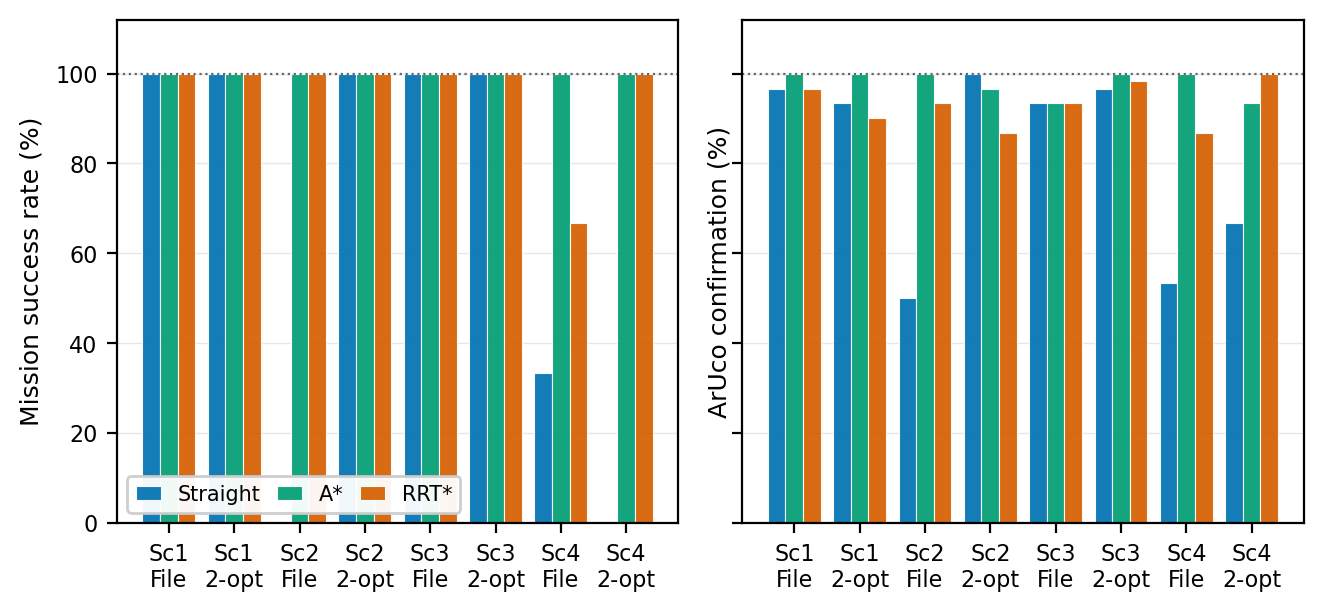
\includegraphics[width=\textwidth]{report_figs/fig_reliability.png}
  \caption{Success and ArUco confirmation by condition. Straight-line flight reaches 0\% success in two conditions; A\textsuperscript{*} completes every run of all eight.}
  \label{fig:reliability}
\end{figure}

\subsection{Discussion}

\paragraph{Ordering dominates, and it is now isolated.} Nine of the twelve ordering comparisons pit two fully-successful configurations against each other; the other three involve a baseline that never completed and are excluded, for the reason given below. Across those nine, NN+2-opt reduces path length by 38.5--49.5\% in Scenarios~1--3 (Figure~\ref{fig:paths}) and cuts tour time in every one, by 3.9\,s to 88.3\,s. Scenario~4 barely moves at $-4$\%: with five viewpoints there is almost nothing left to reorder. This is the largest effect I measured, and unlike the earlier confounded comparison it belongs to ordering alone.

\paragraph{Local planners cost time and distance.} Restricting again to comparisons where both configurations completed, A\textsuperscript{*} \emph{lengthens} the path in all five (+4.4 to +8.8\,m) and increases tour time in all five, by 5.2\,s to 40.4\,s. RRT\textsuperscript{*} behaves identically (+2.3 to +9.1\,m, +1.7 to +42.0\,s). This is the expected price of routing around obstacles rather than through them. Read on time alone, the obstacle-aware planners look strictly worse than straight-line flight, and the earlier confounded design concealed this by crediting the planner with the ordering's gains.

\paragraph{The planners buy completion, not speed.} Figure~\ref{fig:reliability} makes the point directly. Straight-line flight fails outright where obstacles obstruct viewpoints: 0\% success in Scenario~2 under file ordering, and 33\% and 0\% in Scenario~4. A\textsuperscript{*} completes every run in all eight conditions; RRT\textsuperscript{*} completes all but Scenario~4 under file ordering (67\%). Obstacle-aware planning therefore does not make the drone faster, it converts an unreliable system into a reliable one for a modest time cost. Scenario~4 looks like an exception, since A\textsuperscript{*} records 73.4\,s against the baseline's 77.3\,s, but that baseline never finished a single run and its timing is no more comparable than its distance.

\paragraph{Read success before distance.} Scenario~2 file-order straight-line records 105.4\,m against A\textsuperscript{*}'s 156.0\,m, which looks decisive until coverage is read: it visited 53\% of viewpoints. It flew less because it did less. Any comparison involving a sub-100\% cell is void, which is why those cells are daggered in Table~\ref{tab:results}.

\paragraph{A\textsuperscript{*} versus RRT\textsuperscript{*}.} Their paths sit within 1\,m of each other in most cells, so the continuous-space advantage I expected from RRT\textsuperscript{*} never appeared at 3000 samples per segment. On time they trade places by scenario, mostly inside one standard deviation, and several cells carry deviations of 8--47\,s, so I report those gaps as ties rather than results. On reliability A\textsuperscript{*} is the clear choice: it alone completed all 24 of its runs, whereas RRT\textsuperscript{*} lost a third of its Scenario~4 file-order runs with a spread of $\pm46.8$\,s, consistent with its sampling struggling in fragmented free space.

\subsection{Limitations and Improvements}

The 0.5\,m voxel treats any obstacle-adjacent cell as blocked regardless of true clearance, forcing wide detours in Scenario~4; an adaptive octree would refine resolution only near surfaces. Three runs per cell resolves large effects but leaves 5--10\,s differences ambiguous. No collision instrumentation exists, so obstacle strikes were inferred from altitude traces and watchdog aborts rather than measured; a clearance sensor would make the safety claim quantitative. RRT\textsuperscript{*}'s sample budget was fixed at 3000 and never tuned, which plausibly explains why it failed to beat A\textsuperscript{*} on path length. Finally, both planners emit waypoint sequences the controller executes with a stop at each transition; minimum-snap trajectory generation~\cite{mellinger2011minimum} would smooth the velocity profile across the whole tour.

% ─────────────────────────────────────────────────────────────────────────────
\section{Conclusions}
% ─────────────────────────────────────────────────────────────────────────────

A $2\times3$ factorial over four scenarios, 72 runs, separates two effects that a conventional comparison conflates. Tour ordering drives efficiency: NN+2-opt cuts path length by 38--50\% and tour time in every valid comparison. Obstacle-aware planning does the opposite, adding 4--9\,m and 5--40\,s, yet it is the reason the mission finishes at all, lifting success from 0\% to 100\% where straight-line flight fails. The two are complementary, not competing, and a system tuned on time alone would have picked the configuration that never completes the job. For an inspection client this matters more than the seconds: an unfinished survey has no value, however quickly it was flown.

A\textsuperscript{*} is the better default of the two planners: path quality indistinguishable from RRT\textsuperscript{*} here, comparable time, and the only planner to complete all 24 of its runs. Future work should tune the RRT\textsuperscript{*} sample budget before concluding anything about continuous-space planning, add clearance instrumentation, and apply kinodynamic trajectory optimisation to recover the time avoidance costs.

\bibliographystyle{IEEEtran}
\bibliography{references}

\end{document}
